%-------------------------------
% Importer les packages et options du document
%-------------------------------
\documentclass[11pt]{article}
\usepackage[utf8]{inputenc}

\usepackage[utf8]{inputenc}
\usepackage[french]{babel}
\usepackage [T1] {fontenc}

% Geometry
\usepackage{geometry}
\geometry{a4paper}
\geometry{margin=2.5cm}
\setlength{\parskip}{1em}

% Autres
\usepackage{verbatim}
\usepackage{tcolorbox}
\usepackage{tabularx}
\usepackage{multirow}
\usepackage{tabto}
\usepackage{float}
\usepackage{amsfonts}
\usepackage{amsmath}
\usepackage{amssymb}
\usepackage{stmaryrd}
\usepackage{tikz}
\usepackage{pgfplots}
\usepackage{listings}

% Hypper links package and it's configuration
\usepackage{hyperref}
\hypersetup{
    colorlinks=true,
    linkcolor=black,
    filecolor=magenta,
    urlcolor=cyan,
}

%-------------------------------
% Commandes custom
%-------------------------------
% Commande de saut, \myjump{taille du saut en cm} ou \myjump sans arguments
\newcommand{\myjump}[1][0]{\mbox{}\\[#1cm]}

% Pour faire une liste avec des paragraphes
%\biglist{Titre du paragraphe} suite du paragraphe
\newcommand{\biglist}[1]{\myjump[0]\indent\textsc{\textbf{#1}}}
\newcommand{\scbf}[1]{\textsc{\textbf{#1}}}


% Pour faire un commentaire à propos de ce qui devrait être écrit
%\mycomment{Commentaire}
\newcommand{\mycomment}[1]{
\begin{center}
    \small\sc
    [#1]
\end{center}
}

% Pour inclure une figure, elle sera automatiquement numérotée
% \myfigure{chemin ver l'image}{Titre}
\newcounter{nbFigures}
\setcounter{nbFigures}{1}
 \newcommand{\myfigure}[2]{
\begin{center}
    \fbox{
    \includegraphics[width=0.8\linewidth]{#1}}\newline
    \emph{Figure \arabic{nbFigures} : #2}
    \stepcounter{nbFigures}
\end{center}
}

% Pour écrire des ensembles finis de la forme [[a; b]], requiet stmaryrd
\newcommand{\finset}[2]{\ensuremath{\llbracket\,#1;\;#2\,\rrbracket}}

%--------------------------------
% Options de la page de garde, début du document, table des matière
%--------------------------------
\title{\textbf{Dossier d'Analyse Conception}}
\author{Adrien Burgun, Oscar Dewasmes}
\date{UTBM - IT45 - Printemps 2022} % Si commenté, date du jour est utilisé


\begin{document}

\maketitle


\newpage
\tableofcontents


\newpage
\section{Introduction}

Ce document est un rapport d'analyse conception préparant la réalisation du projet d'IT45 printemps 2022 à l'UTBM. Ce projet est réslisé par \emph{Adrien Burgun} et \emph{Oscar Dewasmes}. L'objectif est de mettre en place un algorithme de recherche optimisation pour résoudre un problème d'emplois du temps pour les intervenants du SESSAD.

Le code source du projet ainsi que de ce documents sont disponibles sur \emph{Github} :\newline \href{https://github.com/kalharko/it45-project}{github.com/kalharko/it45-project}

% Expliquer vite-fait le problème

\newpage
\section{Analyse}

% Enlever cette partie?

\subsection{Paramètres}

% TODO: définir des macros pour diminuer l'espace entre les lettres des variables à deux lettres

Nous avons identifié les paramètres suivants :
\begin{itemize}
    \item $n$ \tabto{2cm} le nombre d'agents du SESSAD
    \item $m$ \tabto{2cm} le nombre de missions à réaliser dans une semaine
    \item $v$ \tabto{2cm} la vitesse de déplacement des agents
    \item $CA_i$ \tabto{2cm} la compétence que possède l'agent i
    \item $SA_i$ \tabto{2cm} la spécialité de l'agent i
    \item $CM_j$ \tabto{2cm} la compétence nécessaire à la mission i
    \item $DM_j$ \tabto{2cm} la date du début de la mission $j$
    \item $FM_j$ \tabto{2cm} la date de la fin de la mission $j$
    \item $VH_i$ \tabto{2cm} le volume horaire de l'agent i
\end{itemize}


\subsection{Variables}





Nous avons décidé de représenter une solution par une matrice binaire, dans la quelle chaque colonne représente une mission et chaque ligne représente un agent.

\begin{center}
\begin{tabular}{|c|c c c c|}
\hline
    & $m_0$ & $m_1$ & $\dots$ & $m_o$ \\\hline
    $a_0$ & 1 & 0 & $\dots$ & 1 \\
    $a_1$ & 0 & 1 & $\dots$ & 0 \\
    $\vdots$ & $\vdots$ & $\vdots$ & & $\vdots$\\
    $a_n$ & 0 & 0 & $\dots$ & 0 \\\hline
\end{tabular}
\end{center}


\subsection{Objectifs}


\begin{itemize}
    \item Harmoniser la charge de travail et la distance parcourue entre les agents du SESSAD.
    \item Minimiser le nombre d'affectation qui où l'agent n'a pas la bonne spécialité.
    \item Minimiser le nombre d'heures supplémentaires, le nombre d'heures perdus et la distance totale parcouru.
\end{itemize}



\subsection{Contraintes}

% Soit $CM_i$ la compétence requise pour la mission $i$ et $CA_j$ la compétence de l'agent $j$.

Pour une solution $S \in \mathcal{M}_{n \times o}(\left\{0, 1\right\})$, on a les contraintes suivantes:

\begin{enumerate}
    \item Une mission ne peut être assignée qu'à un intervenant ayant la même compétence: $\forall (i, j), S_{ij} \Rightarrow CM_i = CA_j$
    \item Chaque intervenant ne peut réaliser qu'une mission à la fois: $\forall i, \forall (j_1, j_2), S_{ij_1} \land S_{ij_2} \Rightarrow DM_{j_1} \geq FM_{j_2} + v\Delta_{j_1 j_2} \lor DM_{j_2} \geq FM_{j_1} + v\Delta_{j_1 j_2}$
    \item Une mission est réalisée par un et un seul intervenant: $\forall i, \sum_{j=0}^n{S_{ij}} = 1$
    \item Accorder à chaque intervenant au moins une heure de pause midi par jour entre midi et 14h.
    Pour vérifier cette condition, on regarde l'heure de fin de la dernière mission avant 13h et l'heure de début de la première mission après 13h, et on s'assure qu'il y a au moins une heure entre les deux (en prenant compte du temps de trajet):
    \begin{align*}
        \delta^d_{i,t} =& \min_j(DM_j | S_{ij} \land \text{heure}(DM_j) \geq 13 \land \text{jour}(DM_j) = t) \\
        \delta^f_{i,t} =& \max_j(FM_j + v\Delta_{j,j+1} | S_{ij} \land \text{heure}(FM_j) \leq 13 \land \text{jour}(FM_j) = t) \\
        \forall (i, t),\; &\delta^d_{i,t} - \delta^f_{i,t} \geq 1
    \end{align*}
    \item Respecter les heures maximales à travailler par semaine ($VH_i$, pour lesquelles on compte le temps de la mission ainsi que le temps de trajet): \begin{align*}
        \forall (i, t), T(i, t) &=
            \sum_{j=0}^{n-1} \left\{FM_j - DM_j \;|\; S_{ij} \land \text{jour}(FM_j) = t \right\} \\
            &+ \sum_{j=0,j'=0}^{\min(j,j') \leq n-1} \left\{ v\Delta_{jj'} \;|\; j \neq j' \land S_{ij} \land S_{ij'} \land \text{jour}(FM_j) = t \right\} \\
            &+ v\Delta_{0,jmin} \quad \text{Avec:} \; jmin = \arg\min_j\left\{DM_j \;|\; S_{ij} \land \text{jour}(FM_j) = t
            \right\} \\
            &+ v\Delta_{jmax,0} \quad \text{Avec:} \; jmax = \arg\max_j\left\{FM_j \;|\; S_{ij} \land \text{jour}(FM_j) = t
            \right\} \\
        \forall i, \sum_t T(i, t) &\leq VH_i
    \end{align*}
    \item Respecter les heures maximales à travailler par jour: $\forall (i, t), T(i, t) \leq 10$
    \item Respecter la limite des heures supplémentaires autorisées: $\forall i, \sum_t \max\{T-8,0\} = 10$
    \item Respecter l'amplitude de la journée de travail de chaque intervenant: \begin{align*}
        \forall (i, t),
            \;& \max_j\left\{FM_j \;|\; S_{ij} \land \text{jour}(FM_j) \right\} \\
            -& \min_j\left\{DM_j \;|\; S_{ij} \land \text{jour}(DM_j) \right\} \\
            +&\, v\Delta_{0,jmin} + v\Delta_{jmax,0} \leq 12
    \end{align*}
\end{enumerate}


% 2. Une mission ne peut ˆetre assign ́ee qu’`a un intervenant ayant la mˆeme comp ́etence,
% 3. Chaque Intervenant ne peut r ́ealiser qu’une mission `a la fois,
% 4. Une mission est r ́ealis ́ee par un et un seul Intervenant,
% 5. Accorder `a chaque intervenant au moins une heure de pause-midi par jour entre midi et 14h,
% 6. Respecter les heures maximales `a travailler par jour (Temps Plein = 8h/jour, Temps partiel =
% 6h/jour),
% 7. Respecter la limite des heures suppl ́ementaires autoris ́ees `a travailler par les intervenants sur le plan
% de planification (heures suppl ́ementaires = 10h/semaine, 2h/jour),
% 8. Respecter l’amplitude de la journ ́ee de travail de chaque intervenant (amplitude = 12h),
% 9. Un intervenant doit avoir assez de temps pour se d ́eplacer d’une mission `a une autre.




\newpage
\section{Conception}

Nous avons décidé de réaliser ce projet en c.


\subsection{Algorithme}

Nous allons implémenter l'algorithme du \emph{recuit}. Pour cela nous allons avoir besoin de déterminer une solution finale, une fonction d'évaluation et un moyen de déterminer les voisins d'une solution.


\subsubsection{Solution initiale}

Pour pouvoir initier l'algorithme du \emph{recuit}, il faut déterminer une solution initiale.
Pour cela, nous utilisons une forme relaxée des règles:

\begin{itemize}
    \item Une mission peut ne pas être réalisée
    \item Deux missions pour un agent peuvent se chevaucher
    \item On peut dépasser les heures maximales à travailler par jour
    \item On peut dépasser la limite des heures supplémentaires autorisées
    \item On peut ne pas respecter l'amplitude de la journée de travail
\end{itemize}

On commence par affecter à tous les agent du SESSAD une mission par jour qui convient parfaitement à leur compétences et leur spécialité.
Puis nous répétons le processus jusqu'à ce que l'on ne puisse plus faire d'affectation.
De la même manière, on affecte ensuite aux agents du SESSAD des missions non optimales où leur spécialité ne correspond pas.
Lorsque l'on ne peut à nouveau plus faire d'affectation, on vérifie si les conditions sont toutes remplies.
Si elles le sont, alors on prend cette solution comme solution initiale et on procède à la suite de l'algorithme.

Si une ou plusieurs conditions ne sont pas remplies, alors on procède à chercher une solution initiale par algorithme génétique:

\begin{itemize}
    \item Le génome est constitué de $n$ gènes $g_j \in Agents \cup \{ \varnothing \}$
    \item On convertit chaque génome $g$ en une solution $S$ avec la relation $S_{ij} \Leftrightarrow g_j = i$
    \item On donne un score à chaque individu: si la solution $S$ ne remplit pas les règles relaxées, alors il obtient une pénalité de $\infty$; sinon, elle obtient une pénalité proportionnelle au temps dépassant les limites des règles strictes et au nombre de missions non-réalisées
    \item On élimine tous les individus ayant une pénalité de $\infty$, ainsi que les individus ayant la plus haute pénalité
    \item Une partie des meilleurs individus obtient le droit de se reproduire: l'opérateur de croisement revient à choisir un jour $t$ et à échanger les gènes de ce jour: $\left\{g_j \;|\; \text{jour}(FM_j) = t \right\}$
    \item L'étape de mutation se fait en modifiant un ou plusieurs gènes
    \item Un faible nombre d'individus neufs sont introduits, afin de maintenir la diversité du bassin génétique
\end{itemize}

Une fois que le meilleur individu a un score nul, on le choisit comme solution initiale.

\subsubsection{Fonction d'évaluation}

La fonction d'évaluation se sépare en 2 étapes, la vérification de la validité de la solution puis l'évaluation de la solution par rapport aux objectifs. Pour vérifier la validité de la solution, nous allons vérifier les contraintes une à unes.\newline

Pour évaluer la solution nous pouvons prendre en compte ses caractéristiques suivantes :
\begin{itemize}
    \item $c_0$ = Nombre de mission assignées
    \item $c_1$ = Nombre de missions assignées à un agent qui n'a pas la bonne spécialité
    \item $c_2$ = Nombre d'heures supplémentaires
    \item $c_3$ = Distance totale parcourue
\end{itemize}
\tabto{1.3cm}$\vdots$

Ainsi le score d'une solution serait calculé ainsi :\newline
\tabto{2cm} $score = \lambda_0 c_0 + \lambda_1 c_1 + \lambda_2 c_2 + \dots +\lambda_n c_n$ \newline
Avec $\lambda_i$ l'importance que nous assignons au critère $i$. Par exemple le nombre d'heure supplémentaire est un critère que nous voulons beaucoup minimiser, ainsi son $\lambda$ associé serait une grande valeur négative.



\subsubsection{Déterminer les voisins d'une solution}

Pour déterminer une solution voisine à la solution actuel, une mission et un agent sont choisis au hasard. Cet agent remplace celui qui était affecté précédemment à la mission. Si cette nouvelle affectation n'est pas valide, une nouvelle mission et un nouvel agent sont tirés au hasard jusqu'à ce que une affectation valide apparaisse.


\newpage
\subsubsection{Algorithme du recuit}

\myfigure{Images/Flowchart_recuit.pdf}{Flow chart représentant l'exécution de l'algorithme du recuit}

Le flow chart ci-dessus représente les étapes constituant l'algorithme du \emph{recuit}. À cause de l'étape de sélection d'un voisin aléatoire et l'acceptation de la prochaine solution basé sur une probabilité; cet algorithme peut donner différents résultats. C'est pour cela qu'il est appliqué plusieurs fois à un même problème, pour contrecarrer la possibilité d'aberrances probabilistes qui nous éloigneraient de la solution optimale.






\newpage
\section{Réalisation}

\noindent Par rapport à notre analyse initiale, nous avons ajusté notre approche sur les points suivants :
\begin{itemize}
    \item Évaluation multi-objetif en cascade au lieu de moyenne pondérée.
    \item La solution est maintenant représenté par une liste d'assignation $x_i = j$ où la mission $i$ est assigné à l'agent $j$.
    \item Certaines contraintes, comme l'assignation unique d'une solution, sont directement prises en compte par la forme de la solution.
    \item Pour palier à la nature aléatoire du \emph{recuit}, l'optimisation peut être lancée plusieurs fois pour garder la meilleur solution.
\end{itemize}


\myjump
Nous avons aussi instauré des test unitaires en utilisant la librairie \emph{unity}. Cela nous a permit de s'assurer de la qualité du code que nous avons écrit.

\myjump
La dernière mesure que nous avons prise pour s'assurer de la qualité du code est l'utilisation de \emph{valgrind} qui permet la détection des fuites de mémoire.



\section{Résultats}

Notre programme est capable de trouver une solution initiale pour les 3 instances du problèmes fournies.

Sur l'instance \og 45-4 \fg, nous obtenons comme solution:

\begin{table}[H]
    \centering
    \begin{tabular}{c|c c|c}
        mission & agent & mission & agent \\
        \hline
        1 & 1 & 26 & 2 \\
        2 & 3 & 27 & 1 \\
        3 & 1 & 28 & 3 \\
        4 & 1 & 29 & 1 \\
        5 & 3 & 30 & 3 \\
        6 & 0 & 31 & 0 \\
        7 & 2 & 32 & 2 \\
        8 & 2 & 33 & 0 \\
        9 & 0 & 34 & 2 \\
        10 & 1 & 35 & 0 \\
        11 & 3 & 36 & 1 \\
        12 & 1 & 37 & 3 \\
        13 & 3 & 38 & 3 \\
        14 & 2 & 39 & 3 \\
        15 & 0 & 40 & 1 \\
        16 & 0 & 41 & 2 \\
        17 & 2 & 42 & 0 \\
        18 & 0 & 43 & 2 \\
        19 & 3 & 44 & 0 \\
        20 & 1 & 45 & 2 \\
        21 & 3 & & \\
        22 & 1 & & \\
        23 & 2 & & \\
        24 & 0 & & \\
        25 & 0 & & \\
    \end{tabular}
    \caption{Une solution finale pour 45-4}
    \label{tab:45-4}
\end{table}

La distance totale parcourue est de $423.7$ km et $28$ affectations ont la mauvaise spécialité.
Les scores à optimiser ont pour valeur:

\begin{itemize}
    \item $f_{\text{employees}} = 0.587$
    \item $f_{\text{students}} = 60.0$
    \item $f_{\text{SESSAD}} = 484.87$
\end{itemize}

Pour le problème \og 100-10 \fg, on obtient une solution avec une distance totale parcourue de $1096$ km et $72$ affectations avec la mauvaise spécialité.
Les scores sont:

\begin{itemize}
    \item $f_{\text{employees}} = 1.129$
    \item $f_{\text{students}} = 72.0$
    \item $f_{\text{SESSAD}} = 911.37$
\end{itemize}

\subsection{Taux de succès des fonctions d'initialisation}

Nous avons mesuré le taux de succès des deux fonctions d'initialisation (l'heuristique \og naïve \fg et l'algorithme génétique), en fonction du nombre d'agents et du nombre de missions.
Plus précisément, nous mesurons
$$
\text{perf} = \mathbb{E}(\text{valid}(f(X, \text{Seed})) \;\vert\; \varepsilon)
$$
Avec $X$ un problème suivant une loi uniforme pour les compétences, spécialisations, horaires et durées; $f$ la fonction donnant une solution initiale à mesurer et $\varepsilon = (\texttt{n\_agents}, \texttt{n\_missions})$

Pour $f_1 = \texttt{build\_naive}$ (heuristique seulement), on obtient la distribution suivante:

\begin{figure}[H]
    \centering
    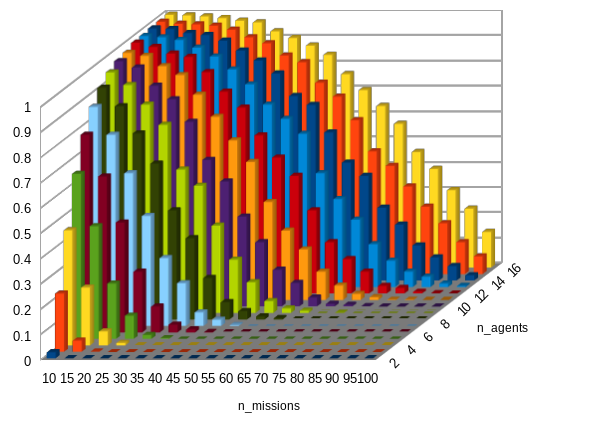
\includegraphics[width=0.75\textwidth]{Images/naive.png}
    \caption{Taux de succès de \texttt{build\_naive}}
    \label{fig:naive_success}
\end{figure}

Pour $f_2 = \texttt{build\_initial\_solution}$ (algorithme génétique), on obtient la distribution suivante:

\begin{figure}[H]
    \centering
    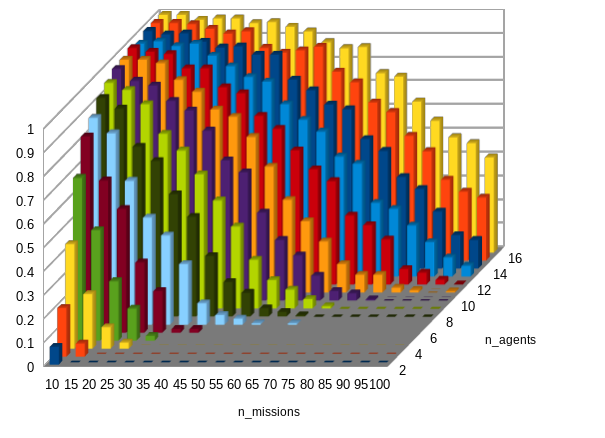
\includegraphics[width=0.75\textwidth]{Images/initial.png}
    \caption{Taux de succès de \texttt{build\_initial\_solution}}
    \label{fig:initial_success}
\end{figure}

Et voici la distribution de $\mathbb{E}(\neg \text{valid}(f_1(X, \text{Seed})) \land \text{valid}(f_2(X, \text{Seed})) \;\vert\; \varepsilon)$, qui représente la contribution de l'algorithme génétique à trouver une solution initiale:

\begin{figure}[H]
    \centering
    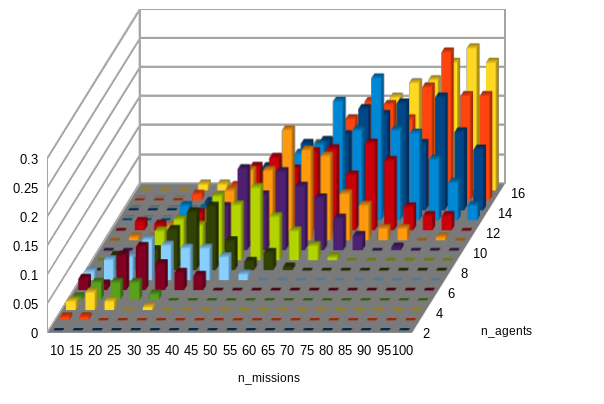
\includegraphics[width=0.75\textwidth]{Images/initial-diff.png}
    \caption{Différence du taux de succès de \texttt{build\_naive} et \texttt{build\_initial\_solution} (échelle ré-ajustée)}
    \label{fig:diff_success}
\end{figure}

\subsection{Évolution des objectifs au cours de la résolution}

Ci dessous est représenté l'évolution des objectifs au fil des itérations. Les barres verticales représentent le changement d'objectif dans la cascade.

\begin{figure}[H]
    \centering
    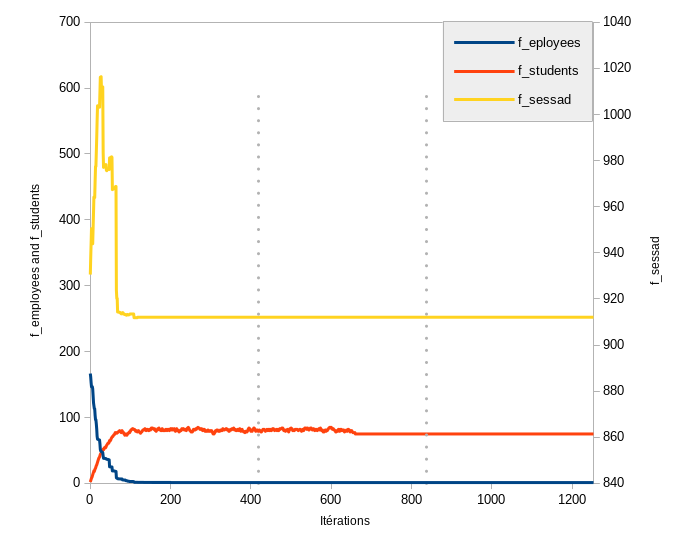
\includegraphics[width=0.8\textwidth]{Images/score_evolution_graph.png}
    \caption{Évolution des objectifs au fil des itérations}
    \label{fig:score_evolution}
\end{figure}

\begin{figure}[H]
    \centering
    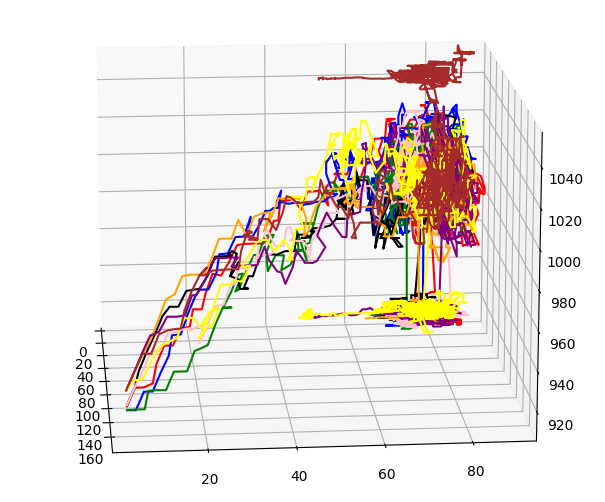
\includegraphics[width=0.75\textwidth]{Images/3d_visualisation.png}
    \caption{Représentation du chemin suivi par 10 solutions initiales différentes lors de l'optimisation}
    \label{fig:score_3d}
\end{figure}

\subsection{Visualisations de la solution}

\begin{figure}[H]
    \caption{Chemin tracé par les agents dans la solution initiale ($\Sigma = 1063.87 \pm 15.15$ km)}
    \center
\begin{tikzpicture}
  \node[rectangle,fill,inner sep=1pt] at (0, 0) (0) {};
    \node[circle,fill,inner sep=1pt] at (0.230759044154621, -1.6625575369947878) (1) {};
    \node[circle,fill,inner sep=1pt] at (2.82041274510218, 1.5569952541596608) (2) {};
    \node[circle,fill,inner sep=1pt] at (1.3066385613759428, -0.16280550788842246) (3) {};
    \node[circle,fill,inner sep=1pt] at (-3.3766152411186074, -1.554984179629346) (4) {};
    \node[circle,fill,inner sep=1pt] at (-2.0677004515697437, -2.5923203631419303) (5) {};
    \node[circle,fill,inner sep=1pt] at (3.667697344423089, -3.2366538034255026) (6) {};
    \node[circle,fill,inner sep=1pt] at (-1.040086713433326, 2.5066137114905223) (7) {};
    \node[circle,fill,inner sep=1pt] at (3.650923312956254, 1.3600845060415079) (8) {};
    \node[circle,fill,inner sep=1pt] at (0.6231538405101776, -2.3663358253066398) (9) {};
    \node[circle,fill,inner sep=1pt] at (-1.196566321929575, -1.6204463921312033) (10) {};
    \node[circle,fill,inner sep=1pt] at (0.5309499466470191, -2.8199337346951725) (11) {};
    \node[circle,fill,inner sep=1pt] at (0.0041393874677694694, 0.8298564204977102) (12) {};
    \node[circle,fill,inner sep=1pt] at (4.103812743212403, -2.280170731024778) (13) {};
    \node[circle,fill,inner sep=1pt] at (-0.024898335178615998, -4.68227174457932) (14) {};
    \node[circle,fill,inner sep=1pt] at (0.2977236929704869, -1.8035928443521554) (15) {};
    \node[circle,fill,inner sep=1pt] at (1.6089293304751118, 0.34205846889330266) (16) {};
    \node[circle,fill,inner sep=1pt] at (2.0854774802242164, -2.1595119438029515) (17) {};
    \node[circle,fill,inner sep=1pt] at (1.3605837127292166, -1.8884475372555993) (18) {};
    \node[circle,fill,inner sep=1pt] at (-3.883458619364125, -0.04679921698860873) (19) {};
    \node[circle,fill,inner sep=1pt] at (-0.05002142737837225, 0.15153471956246936) (20) {};
    \node[circle,fill,inner sep=1pt] at (-2.615265028019659, -1.4741781520643067) (21) {};
    \node[circle,fill,inner sep=1pt] at (-3.563460702923992, 3.0829685867360572) (22) {};
    \node[circle,fill,inner sep=1pt] at (1.2345658592980753, 0.3150532447197752) (23) {};
    \node[circle,fill,inner sep=1pt] at (-3.6125576410491522, -3.309564216471854) (24) {};
    \node[circle,fill,inner sep=1pt] at (2.5701989122667803, 1.4666619287005846) (25) {};
    \node[circle,fill,inner sep=1pt] at (2.5953721021033456, 1.5989318198251774) (26) {};
    \node[circle,fill,inner sep=1pt] at (4.261571405333174, -2.504605981945409) (27) {};
    \node[circle,fill,inner sep=1pt] at (1.9917404067351763, -0.5157853879755964) (28) {};
    \node[circle,fill,inner sep=1pt] at (0.7668810712724169, -0.4866142409695547) (29) {};
    \node[circle,fill,inner sep=1pt] at (0.012697065452541834, -2.699269248158551) (30) {};
    \node[circle,fill,inner sep=1pt] at (0.21629901569586452, -5.040383065419475) (31) {};
    \node[circle,fill,inner sep=1pt] at (-1.8537506426816088, -3.0764225268226633) (32) {};
    \node[circle,fill,inner sep=1pt] at (1.5300832054091509, 3.1713079366242196) (33) {};
    \node[circle,fill,inner sep=1pt] at (2.150192184198767, 3.989898509386318) (34) {};
    \node[circle,fill,inner sep=1pt] at (-3.3779501754335524, 3.6618114407607316) (35) {};
    \node[circle,fill,inner sep=1pt] at (1.9977873843003202, 2.9316960153538414) (36) {};
    \node[circle,fill,inner sep=1pt] at (-1.0982153364289338, 3.460309455073223) (37) {};
    \node[circle,fill,inner sep=1pt] at (-0.1481083285557554, 2.2175039014928406) (38) {};
    \node[circle,fill,inner sep=1pt] at (3.070916015330287, -0.9616171308799488) (39) {};
    \node[circle,fill,inner sep=1pt] at (4.787977631369486, -0.012424211898620722) (40) {};
    \node[circle,fill,inner sep=1pt] at (3.597677348263957, 0.47977930039972605) (41) {};
    \node[circle,fill,inner sep=1pt] at (4.576041994840474, -1.4647057431900692) (42) {};
    \node[circle,fill,inner sep=1pt] at (0.6334684203331684, -2.0031911797268624) (43) {};
    \node[circle,fill,inner sep=1pt] at (4.466182869166802, 1.4405043271267033) (44) {};
    \node[circle,fill,inner sep=1pt] at (-0.4263087918396467, -2.4626478578477307) (45) {};
    \node[circle,fill,inner sep=1pt] at (-4.366419881216976, 0.5142737987548801) (46) {};
    \node[circle,fill,inner sep=1pt] at (-0.8989947823938288, 2.016380068640787) (47) {};
    \node[circle,fill,inner sep=1pt] at (0.401610090006337, 4.959616934580525) (48) {};
    \node[circle,fill,inner sep=1pt] at (2.1020403802445884, 2.5456893490209276) (49) {};
    \node[circle,fill,inner sep=1pt] at (-0.708115647543749, 1.814938547455922) (50) {};
    \node[circle,fill,inner sep=1pt] at (-2.5418151400636555, -2.1855185074446677) (51) {};
    \node[circle,fill,inner sep=1pt] at (-2.7803624836336702, -3.040853352880549) (52) {};
    \node[circle,fill,inner sep=1pt] at (-3.684447585945104, -3.016756139881446) (53) {};
    \node[circle,fill,inner sep=1pt] at (-1.9279637749578433, -4.293344677279276) (54) {};
    \node[circle,fill,inner sep=1pt] at (3.4988282710706735, 2.7208073622379874) (55) {};
    \node[circle,fill,inner sep=1pt] at (-1.6809128227974424, 1.8629094522149585) (56) {};
    \node[circle,fill,inner sep=1pt] at (3.824581992513406, -0.9722529297688794) (57) {};
    \node[circle,fill,inner sep=1pt] at (-2.697896647107651, 3.8431749245177746) (58) {};
    \node[circle,fill,inner sep=1pt] at (1.4335366239876453, 1.4781884066600341) (59) {};
    \node[circle,fill,inner sep=1pt] at (0.7844755904088765, 1.6959424193599808) (60) {};
    \node[circle,fill,inner sep=1pt] at (-0.5190214949493063, -3.888994620116117) (61) {};
    \node[circle,fill,inner sep=1pt] at (1.5804787742797777, -1.0442481303006779) (62) {};
    \node[circle,fill,inner sep=1pt] at (-3.635493136779917, -1.392560433465738) (63) {};
    \node[circle,fill,inner sep=1pt] at (-3.5736391127690683, 0.7314712375857744) (64) {};
    \node[circle,fill,inner sep=1pt] at (-4.652701969835232, -1.040374045175357) (65) {};
    \node[circle,fill,inner sep=1pt] at (3.6210328758824986, -2.357984493475437) (66) {};
    \node[circle,fill,inner sep=1pt] at (0.9938528715174366, -0.029191695497291704) (67) {};
    \node[circle,fill,inner sep=1pt] at (-2.282757088706418, 2.3844849354784117) (68) {};
    \node[circle,fill,inner sep=1pt] at (2.0291321982033867, 0.8643587243258428) (69) {};
    \node[circle,fill,inner sep=1pt] at (3.1662199705287, 0.4528805402385833) (70) {};
    \node[circle,fill,inner sep=1pt] at (-1.4899138734296349, -3.5897728122622077) (71) {};
    \node[circle,fill,inner sep=1pt] at (-2.759289750834009, -2.7404115932457924) (72) {};
    \node[circle,fill,inner sep=1pt] at (0.5130547137976901, -0.38210653082215834) (73) {};
    \node[circle,fill,inner sep=1pt] at (-3.972316628213975, -3.1284886841241053) (74) {};
    \node[circle,fill,inner sep=1pt] at (-3.9789977431102157, 1.8872387364404404) (75) {};
    \node[circle,fill,inner sep=1pt] at (3.6425330755620777, 0.5770603808885695) (76) {};
    \node[circle,fill,inner sep=1pt] at (3.0733244483211495, 0.14793257143162888) (77) {};
    \node[circle,fill,inner sep=1pt] at (0.1693022699976089, 4.252829778537711) (78) {};
    \node[circle,fill,inner sep=1pt] at (-0.006120751464982503, -1.2847452165671984) (79) {};
    \node[circle,fill,inner sep=1pt] at (3.7611427495142733, -0.3879120827735415) (80) {};
    \node[circle,fill,inner sep=1pt] at (3.372216425205935, 0.7151949877241951) (81) {};
    \node[circle,fill,inner sep=1pt] at (-4.598633039311766, 1.4633569315764816) (82) {};
    \node[circle,fill,inner sep=1pt] at (-3.9070044629886747, -1.0134671384958625) (83) {};
    \node[circle,fill,inner sep=1pt] at (2.948664327479149, -1.5912145014931205) (84) {};
    \node[circle,fill,inner sep=1pt] at (1.3212014139997366, -1.6133616002998643) (85) {};
    \node[circle,fill,inner sep=1pt] at (3.1017592687235593, 2.4239644981153248) (86) {};
    \node[circle,fill,inner sep=1pt] at (0.333229737992979, 4.1978414856068085) (87) {};
    \node[circle,fill,inner sep=1pt] at (-0.7638766640292325, -1.09931671302658) (88) {};
    \node[circle,fill,inner sep=1pt] at (-0.3001781863720503, -2.7656323614494744) (89) {};
    \node[circle,fill,inner sep=1pt] at (4.123695508818637, -0.7673659672496546) (90) {};
    \node[circle,fill,inner sep=1pt] at (-3.3278012980796525, 2.87906733720465) (91) {};
    \node[circle,fill,inner sep=1pt] at (0.26688703718116236, 1.916581024785385) (92) {};
    \node[circle,fill,inner sep=1pt] at (-1.5113294471658976, 4.620714593460826) (93) {};
    \node[circle,fill,inner sep=1pt] at (0.0330939224484987, -1.034882836064076) (94) {};
    \node[circle,fill,inner sep=1pt] at (1.0089916888757942, 1.201169453963833) (95) {};
    \node[circle,fill,inner sep=1pt] at (3.0267301092654777, -1.1174243156418828) (96) {};
    \node[circle,fill,inner sep=1pt] at (4.685034788632226, -0.7271488082241038) (97) {};
    \node[circle,fill,inner sep=1pt] at (2.344294415547571, 2.711714345026223) (98) {};
    \node[circle,fill,inner sep=1pt] at (-3.378264393934195, -2.3975562398647434) (99) {};
    \node[circle,fill,inner sep=1pt] at (1.8344751271403525, 0.9329387781980865) (100) {};
  \draw[draw=black,densely dotted] (0) -- (3);
  \draw[draw=black] (3) -- (16);
  \draw[draw=black,densely dotted] (16) -- (0);
  \draw[draw=black,densely dotted] (0) -- (23);
  \draw[draw=black] (23) -- (36);
  \draw[draw=black,densely dotted] (36) -- (0);
  \draw[draw=black,densely dotted] (0) -- (43);
  \draw[draw=black] (43) -- (56);
  \draw[draw=black,densely dotted] (56) -- (0);
  \draw[draw=black,densely dotted] (0) -- (63);
  \draw[draw=black] (63) -- (76);
  \draw[draw=black,densely dotted] (76) -- (0);
  \draw[draw=black,densely dotted] (0) -- (83);
  \draw[draw=black] (83) -- (96);
  \draw[draw=black,densely dotted] (96) -- (0);
  \draw[draw=magenta,densely dotted] (0) -- (5);
  \draw[draw=magenta] (5) -- (13);
  \draw[draw=magenta,densely dotted] (13) -- (0);
  \draw[draw=magenta,densely dotted] (0) -- (25);
  \draw[draw=magenta] (25) -- (33);
  \draw[draw=magenta,densely dotted] (33) -- (0);
  \draw[draw=magenta,densely dotted] (0) -- (45);
  \draw[draw=magenta] (45) -- (53);
  \draw[draw=magenta,densely dotted] (53) -- (0);
  \draw[draw=magenta,densely dotted] (0) -- (65);
  \draw[draw=magenta] (65) -- (73);
  \draw[draw=magenta,densely dotted] (73) -- (0);
  \draw[draw=magenta,densely dotted] (0) -- (85);
  \draw[draw=magenta] (85) -- (93);
  \draw[draw=magenta,densely dotted] (93) -- (0);
  \draw[draw=cyan,densely dotted] (0) -- (4);
  \draw[draw=cyan] (4) -- (17);
  \draw[draw=cyan,densely dotted] (17) -- (0);
  \draw[draw=cyan,densely dotted] (0) -- (24);
  \draw[draw=cyan] (24) -- (37);
  \draw[draw=cyan,densely dotted] (37) -- (0);
  \draw[draw=cyan,densely dotted] (0) -- (44);
  \draw[draw=cyan] (44) -- (57);
  \draw[draw=cyan,densely dotted] (57) -- (0);
  \draw[draw=cyan,densely dotted] (0) -- (64);
  \draw[draw=cyan] (64) -- (77);
  \draw[draw=cyan,densely dotted] (77) -- (0);
  \draw[draw=cyan,densely dotted] (0) -- (84);
  \draw[draw=cyan] (84) -- (97);
  \draw[draw=cyan,densely dotted] (97) -- (0);
  \draw[draw=olive,densely dotted] (0) -- (7);
  \draw[draw=olive] (7) -- (18);
  \draw[draw=olive,densely dotted] (18) -- (0);
  \draw[draw=olive,densely dotted] (0) -- (27);
  \draw[draw=olive] (27) -- (38);
  \draw[draw=olive,densely dotted] (38) -- (0);
  \draw[draw=olive,densely dotted] (0) -- (47);
  \draw[draw=olive] (47) -- (58);
  \draw[draw=olive,densely dotted] (58) -- (0);
  \draw[draw=olive,densely dotted] (0) -- (67);
  \draw[draw=olive] (67) -- (78);
  \draw[draw=olive,densely dotted] (78) -- (0);
  \draw[draw=olive,densely dotted] (0) -- (87);
  \draw[draw=olive] (87) -- (98);
  \draw[draw=olive,densely dotted] (98) -- (0);
  \draw[draw=violet,densely dotted] (0) -- (10);
  \draw[draw=violet] (10) -- (20);
  \draw[draw=violet,densely dotted] (20) -- (0);
  \draw[draw=violet,densely dotted] (0) -- (30);
  \draw[draw=violet] (30) -- (40);
  \draw[draw=violet,densely dotted] (40) -- (0);
  \draw[draw=violet,densely dotted] (0) -- (50);
  \draw[draw=violet] (50) -- (60);
  \draw[draw=violet,densely dotted] (60) -- (0);
  \draw[draw=violet,densely dotted] (0) -- (70);
  \draw[draw=violet] (70) -- (80);
  \draw[draw=violet,densely dotted] (80) -- (0);
  \draw[draw=violet,densely dotted] (0) -- (90);
  \draw[draw=violet] (90) -- (100);
  \draw[draw=violet,densely dotted] (100) -- (0);
  \draw[draw=blue,densely dotted] (0) -- (8);
  \draw[draw=blue] (8) -- (19);
  \draw[draw=blue,densely dotted] (19) -- (0);
  \draw[draw=blue,densely dotted] (0) -- (28);
  \draw[draw=blue] (28) -- (39);
  \draw[draw=blue,densely dotted] (39) -- (0);
  \draw[draw=blue,densely dotted] (0) -- (48);
  \draw[draw=blue] (48) -- (59);
  \draw[draw=blue,densely dotted] (59) -- (0);
  \draw[draw=blue,densely dotted] (0) -- (68);
  \draw[draw=blue] (68) -- (79);
  \draw[draw=blue,densely dotted] (79) -- (0);
  \draw[draw=blue,densely dotted] (0) -- (88);
  \draw[draw=blue] (88) -- (99);
  \draw[draw=blue,densely dotted] (99) -- (0);
  \draw[draw=brown,densely dotted] (0) -- (2);
  \draw[draw=brown] (2) -- (12);
  \draw[draw=brown,densely dotted] (12) -- (0);
  \draw[draw=brown,densely dotted] (0) -- (22);
  \draw[draw=brown] (22) -- (32);
  \draw[draw=brown,densely dotted] (32) -- (0);
  \draw[draw=brown,densely dotted] (0) -- (42);
  \draw[draw=brown] (42) -- (52);
  \draw[draw=brown,densely dotted] (52) -- (0);
  \draw[draw=brown,densely dotted] (0) -- (62);
  \draw[draw=brown] (62) -- (72);
  \draw[draw=brown,densely dotted] (72) -- (0);
  \draw[draw=brown,densely dotted] (0) -- (82);
  \draw[draw=brown] (82) -- (92);
  \draw[draw=brown,densely dotted] (92) -- (0);
  \draw[draw=red,densely dotted] (0) -- (9);
  \draw[draw=red] (9) -- (15);
  \draw[draw=red,densely dotted] (15) -- (0);
  \draw[draw=red,densely dotted] (0) -- (29);
  \draw[draw=red] (29) -- (35);
  \draw[draw=red,densely dotted] (35) -- (0);
  \draw[draw=red,densely dotted] (0) -- (49);
  \draw[draw=red] (49) -- (55);
  \draw[draw=red,densely dotted] (55) -- (0);
  \draw[draw=red,densely dotted] (0) -- (69);
  \draw[draw=red] (69) -- (75);
  \draw[draw=red,densely dotted] (75) -- (0);
  \draw[draw=red,densely dotted] (0) -- (89);
  \draw[draw=red] (89) -- (95);
  \draw[draw=red,densely dotted] (95) -- (0);
  \draw[draw=orange,densely dotted] (0) -- (1);
  \draw[draw=orange] (1) -- (11);
  \draw[draw=orange,densely dotted] (11) -- (0);
  \draw[draw=orange,densely dotted] (0) -- (21);
  \draw[draw=orange] (21) -- (31);
  \draw[draw=orange,densely dotted] (31) -- (0);
  \draw[draw=orange,densely dotted] (0) -- (41);
  \draw[draw=orange] (41) -- (51);
  \draw[draw=orange,densely dotted] (51) -- (0);
  \draw[draw=orange,densely dotted] (0) -- (61);
  \draw[draw=orange] (61) -- (71);
  \draw[draw=orange,densely dotted] (71) -- (0);
  \draw[draw=orange,densely dotted] (0) -- (81);
  \draw[draw=orange] (81) -- (91);
  \draw[draw=orange,densely dotted] (91) -- (0);
  \draw[draw=pink,densely dotted] (0) -- (6);
  \draw[draw=pink] (6) -- (14);
  \draw[draw=pink,densely dotted] (14) -- (0);
  \draw[draw=pink,densely dotted] (0) -- (26);
  \draw[draw=pink] (26) -- (34);
  \draw[draw=pink,densely dotted] (34) -- (0);
  \draw[draw=pink,densely dotted] (0) -- (46);
  \draw[draw=pink] (46) -- (54);
  \draw[draw=pink,densely dotted] (54) -- (0);
  \draw[draw=pink,densely dotted] (0) -- (66);
  \draw[draw=pink] (66) -- (74);
  \draw[draw=pink,densely dotted] (74) -- (0);
  \draw[draw=pink,densely dotted] (0) -- (86);
  \draw[draw=pink] (86) -- (94);
  \draw[draw=pink,densely dotted] (94) -- (0);
\end{tikzpicture}

\end{figure}

\begin{figure}[H]
    \caption{Chemin tracé par les agents dans la solution finale ($\Sigma = 1096.43 \pm 1.16$ km)}
    \center
\begin{tikzpicture}
  \node[rectangle,fill,inner sep=1pt] at (0, 0) (0) {};
    \node[circle,fill,inner sep=1pt] at (0.230759044154621, -1.6625575369947878) (1) {};
    \node[circle,fill,inner sep=1pt] at (2.82041274510218, 1.5569952541596608) (2) {};
    \node[circle,fill,inner sep=1pt] at (1.3066385613759428, -0.16280550788842246) (3) {};
    \node[circle,fill,inner sep=1pt] at (-3.3766152411186074, -1.554984179629346) (4) {};
    \node[circle,fill,inner sep=1pt] at (-2.0677004515697437, -2.5923203631419303) (5) {};
    \node[circle,fill,inner sep=1pt] at (3.667697344423089, -3.2366538034255026) (6) {};
    \node[circle,fill,inner sep=1pt] at (-1.040086713433326, 2.5066137114905223) (7) {};
    \node[circle,fill,inner sep=1pt] at (3.650923312956254, 1.3600845060415079) (8) {};
    \node[circle,fill,inner sep=1pt] at (0.6231538405101776, -2.3663358253066398) (9) {};
    \node[circle,fill,inner sep=1pt] at (-1.196566321929575, -1.6204463921312033) (10) {};
    \node[circle,fill,inner sep=1pt] at (0.5309499466470191, -2.8199337346951725) (11) {};
    \node[circle,fill,inner sep=1pt] at (0.0041393874677694694, 0.8298564204977102) (12) {};
    \node[circle,fill,inner sep=1pt] at (4.103812743212403, -2.280170731024778) (13) {};
    \node[circle,fill,inner sep=1pt] at (-0.024898335178615998, -4.68227174457932) (14) {};
    \node[circle,fill,inner sep=1pt] at (0.2977236929704869, -1.8035928443521554) (15) {};
    \node[circle,fill,inner sep=1pt] at (1.6089293304751118, 0.34205846889330266) (16) {};
    \node[circle,fill,inner sep=1pt] at (2.0854774802242164, -2.1595119438029515) (17) {};
    \node[circle,fill,inner sep=1pt] at (1.3605837127292166, -1.8884475372555993) (18) {};
    \node[circle,fill,inner sep=1pt] at (-3.883458619364125, -0.04679921698860873) (19) {};
    \node[circle,fill,inner sep=1pt] at (-0.05002142737837225, 0.15153471956246936) (20) {};
    \node[circle,fill,inner sep=1pt] at (-2.615265028019659, -1.4741781520643067) (21) {};
    \node[circle,fill,inner sep=1pt] at (-3.563460702923992, 3.0829685867360572) (22) {};
    \node[circle,fill,inner sep=1pt] at (1.2345658592980753, 0.3150532447197752) (23) {};
    \node[circle,fill,inner sep=1pt] at (-3.6125576410491522, -3.309564216471854) (24) {};
    \node[circle,fill,inner sep=1pt] at (2.5701989122667803, 1.4666619287005846) (25) {};
    \node[circle,fill,inner sep=1pt] at (2.5953721021033456, 1.5989318198251774) (26) {};
    \node[circle,fill,inner sep=1pt] at (4.261571405333174, -2.504605981945409) (27) {};
    \node[circle,fill,inner sep=1pt] at (1.9917404067351763, -0.5157853879755964) (28) {};
    \node[circle,fill,inner sep=1pt] at (0.7668810712724169, -0.4866142409695547) (29) {};
    \node[circle,fill,inner sep=1pt] at (0.012697065452541834, -2.699269248158551) (30) {};
    \node[circle,fill,inner sep=1pt] at (0.21629901569586452, -5.040383065419475) (31) {};
    \node[circle,fill,inner sep=1pt] at (-1.8537506426816088, -3.0764225268226633) (32) {};
    \node[circle,fill,inner sep=1pt] at (1.5300832054091509, 3.1713079366242196) (33) {};
    \node[circle,fill,inner sep=1pt] at (2.150192184198767, 3.989898509386318) (34) {};
    \node[circle,fill,inner sep=1pt] at (-3.3779501754335524, 3.6618114407607316) (35) {};
    \node[circle,fill,inner sep=1pt] at (1.9977873843003202, 2.9316960153538414) (36) {};
    \node[circle,fill,inner sep=1pt] at (-1.0982153364289338, 3.460309455073223) (37) {};
    \node[circle,fill,inner sep=1pt] at (-0.1481083285557554, 2.2175039014928406) (38) {};
    \node[circle,fill,inner sep=1pt] at (3.070916015330287, -0.9616171308799488) (39) {};
    \node[circle,fill,inner sep=1pt] at (4.787977631369486, -0.012424211898620722) (40) {};
    \node[circle,fill,inner sep=1pt] at (3.597677348263957, 0.47977930039972605) (41) {};
    \node[circle,fill,inner sep=1pt] at (4.576041994840474, -1.4647057431900692) (42) {};
    \node[circle,fill,inner sep=1pt] at (0.6334684203331684, -2.0031911797268624) (43) {};
    \node[circle,fill,inner sep=1pt] at (4.466182869166802, 1.4405043271267033) (44) {};
    \node[circle,fill,inner sep=1pt] at (-0.4263087918396467, -2.4626478578477307) (45) {};
    \node[circle,fill,inner sep=1pt] at (-4.366419881216976, 0.5142737987548801) (46) {};
    \node[circle,fill,inner sep=1pt] at (-0.8989947823938288, 2.016380068640787) (47) {};
    \node[circle,fill,inner sep=1pt] at (0.401610090006337, 4.959616934580525) (48) {};
    \node[circle,fill,inner sep=1pt] at (2.1020403802445884, 2.5456893490209276) (49) {};
    \node[circle,fill,inner sep=1pt] at (-0.708115647543749, 1.814938547455922) (50) {};
    \node[circle,fill,inner sep=1pt] at (-2.5418151400636555, -2.1855185074446677) (51) {};
    \node[circle,fill,inner sep=1pt] at (-2.7803624836336702, -3.040853352880549) (52) {};
    \node[circle,fill,inner sep=1pt] at (-3.684447585945104, -3.016756139881446) (53) {};
    \node[circle,fill,inner sep=1pt] at (-1.9279637749578433, -4.293344677279276) (54) {};
    \node[circle,fill,inner sep=1pt] at (3.4988282710706735, 2.7208073622379874) (55) {};
    \node[circle,fill,inner sep=1pt] at (-1.6809128227974424, 1.8629094522149585) (56) {};
    \node[circle,fill,inner sep=1pt] at (3.824581992513406, -0.9722529297688794) (57) {};
    \node[circle,fill,inner sep=1pt] at (-2.697896647107651, 3.8431749245177746) (58) {};
    \node[circle,fill,inner sep=1pt] at (1.4335366239876453, 1.4781884066600341) (59) {};
    \node[circle,fill,inner sep=1pt] at (0.7844755904088765, 1.6959424193599808) (60) {};
    \node[circle,fill,inner sep=1pt] at (-0.5190214949493063, -3.888994620116117) (61) {};
    \node[circle,fill,inner sep=1pt] at (1.5804787742797777, -1.0442481303006779) (62) {};
    \node[circle,fill,inner sep=1pt] at (-3.635493136779917, -1.392560433465738) (63) {};
    \node[circle,fill,inner sep=1pt] at (-3.5736391127690683, 0.7314712375857744) (64) {};
    \node[circle,fill,inner sep=1pt] at (-4.652701969835232, -1.040374045175357) (65) {};
    \node[circle,fill,inner sep=1pt] at (3.6210328758824986, -2.357984493475437) (66) {};
    \node[circle,fill,inner sep=1pt] at (0.9938528715174366, -0.029191695497291704) (67) {};
    \node[circle,fill,inner sep=1pt] at (-2.282757088706418, 2.3844849354784117) (68) {};
    \node[circle,fill,inner sep=1pt] at (2.0291321982033867, 0.8643587243258428) (69) {};
    \node[circle,fill,inner sep=1pt] at (3.1662199705287, 0.4528805402385833) (70) {};
    \node[circle,fill,inner sep=1pt] at (-1.4899138734296349, -3.5897728122622077) (71) {};
    \node[circle,fill,inner sep=1pt] at (-2.759289750834009, -2.7404115932457924) (72) {};
    \node[circle,fill,inner sep=1pt] at (0.5130547137976901, -0.38210653082215834) (73) {};
    \node[circle,fill,inner sep=1pt] at (-3.972316628213975, -3.1284886841241053) (74) {};
    \node[circle,fill,inner sep=1pt] at (-3.9789977431102157, 1.8872387364404404) (75) {};
    \node[circle,fill,inner sep=1pt] at (3.6425330755620777, 0.5770603808885695) (76) {};
    \node[circle,fill,inner sep=1pt] at (3.0733244483211495, 0.14793257143162888) (77) {};
    \node[circle,fill,inner sep=1pt] at (0.1693022699976089, 4.252829778537711) (78) {};
    \node[circle,fill,inner sep=1pt] at (-0.006120751464982503, -1.2847452165671984) (79) {};
    \node[circle,fill,inner sep=1pt] at (3.7611427495142733, -0.3879120827735415) (80) {};
    \node[circle,fill,inner sep=1pt] at (3.372216425205935, 0.7151949877241951) (81) {};
    \node[circle,fill,inner sep=1pt] at (-4.598633039311766, 1.4633569315764816) (82) {};
    \node[circle,fill,inner sep=1pt] at (-3.9070044629886747, -1.0134671384958625) (83) {};
    \node[circle,fill,inner sep=1pt] at (2.948664327479149, -1.5912145014931205) (84) {};
    \node[circle,fill,inner sep=1pt] at (1.3212014139997366, -1.6133616002998643) (85) {};
    \node[circle,fill,inner sep=1pt] at (3.1017592687235593, 2.4239644981153248) (86) {};
    \node[circle,fill,inner sep=1pt] at (0.333229737992979, 4.1978414856068085) (87) {};
    \node[circle,fill,inner sep=1pt] at (-0.7638766640292325, -1.09931671302658) (88) {};
    \node[circle,fill,inner sep=1pt] at (-0.3001781863720503, -2.7656323614494744) (89) {};
    \node[circle,fill,inner sep=1pt] at (4.123695508818637, -0.7673659672496546) (90) {};
    \node[circle,fill,inner sep=1pt] at (-3.3278012980796525, 2.87906733720465) (91) {};
    \node[circle,fill,inner sep=1pt] at (0.26688703718116236, 1.916581024785385) (92) {};
    \node[circle,fill,inner sep=1pt] at (-1.5113294471658976, 4.620714593460826) (93) {};
    \node[circle,fill,inner sep=1pt] at (0.0330939224484987, -1.034882836064076) (94) {};
    \node[circle,fill,inner sep=1pt] at (1.0089916888757942, 1.201169453963833) (95) {};
    \node[circle,fill,inner sep=1pt] at (3.0267301092654777, -1.1174243156418828) (96) {};
    \node[circle,fill,inner sep=1pt] at (4.685034788632226, -0.7271488082241038) (97) {};
    \node[circle,fill,inner sep=1pt] at (2.344294415547571, 2.711714345026223) (98) {};
    \node[circle,fill,inner sep=1pt] at (-3.378264393934195, -2.3975562398647434) (99) {};
    \node[circle,fill,inner sep=1pt] at (1.8344751271403525, 0.9329387781980865) (100) {};
  \draw[draw=black,densely dotted] (0) -- (8);
  \draw[draw=black] (8) -- (20);
  \draw[draw=black,densely dotted] (20) -- (0);
  \draw[draw=black,densely dotted] (0) -- (27);
  \draw[draw=black] (27) -- (37);
  \draw[draw=black,densely dotted] (37) -- (0);
  \draw[draw=black,densely dotted] (0) -- (50);
  \draw[draw=black] (50) -- (56);
  \draw[draw=black,densely dotted] (56) -- (0);
  \draw[draw=black,densely dotted] (0) -- (64);
  \draw[draw=black] (64) -- (78);
  \draw[draw=black,densely dotted] (78) -- (0);
  \draw[draw=black,densely dotted] (0) -- (83);
  \draw[draw=black] (83) -- (100);
  \draw[draw=black,densely dotted] (100) -- (0);
  \draw[draw=magenta,densely dotted] (0) -- (9);
  \draw[draw=magenta] (9) -- (12);
  \draw[draw=magenta,densely dotted] (12) -- (0);
  \draw[draw=magenta,densely dotted] (0) -- (29);
  \draw[draw=magenta] (29) -- (32);
  \draw[draw=magenta,densely dotted] (32) -- (0);
  \draw[draw=magenta,densely dotted] (0) -- (42);
  \draw[draw=magenta] (42) -- (53);
  \draw[draw=magenta,densely dotted] (53) -- (0);
  \draw[draw=magenta,densely dotted] (0) -- (61);
  \draw[draw=magenta] (61) -- (73);
  \draw[draw=magenta,densely dotted] (73) -- (0);
  \draw[draw=magenta,densely dotted] (0) -- (82);
  \draw[draw=magenta] (82) -- (93);
  \draw[draw=magenta,densely dotted] (93) -- (0);
  \draw[draw=cyan,densely dotted] (0) -- (4);
  \draw[draw=cyan] (4) -- (18);
  \draw[draw=cyan,densely dotted] (18) -- (0);
  \draw[draw=cyan,densely dotted] (0) -- (24);
  \draw[draw=cyan] (24) -- (39);
  \draw[draw=cyan,densely dotted] (39) -- (0);
  \draw[draw=cyan,densely dotted] (0) -- (44);
  \draw[draw=cyan] (44) -- (60);
  \draw[draw=cyan,densely dotted] (60) -- (0);
  \draw[draw=cyan,densely dotted] (0) -- (70);
  \draw[draw=cyan] (70) -- (79);
  \draw[draw=cyan,densely dotted] (79) -- (0);
  \draw[draw=cyan,densely dotted] (0) -- (90);
  \draw[draw=cyan] (90) -- (98);
  \draw[draw=cyan,densely dotted] (98) -- (0);
  \draw[draw=olive,densely dotted] (0) -- (7);
  \draw[draw=olive] (7) -- (17);
  \draw[draw=olive,densely dotted] (17) -- (0);
  \draw[draw=olive,densely dotted] (0) -- (23);
  \draw[draw=olive] (23) -- (40);
  \draw[draw=olive,densely dotted] (40) -- (0);
  \draw[draw=olive,densely dotted] (0) -- (47);
  \draw[draw=olive] (47) -- (59);
  \draw[draw=olive,densely dotted] (59) -- (0);
  \draw[draw=olive,densely dotted] (0) -- (68);
  \draw[draw=olive] (68) -- (76);
  \draw[draw=olive,densely dotted] (76) -- (0);
  \draw[draw=olive,densely dotted] (0) -- (84);
  \draw[draw=olive] (84) -- (99);
  \draw[draw=olive,densely dotted] (99) -- (0);
  \draw[draw=violet,densely dotted] (0) -- (3);
  \draw[draw=violet] (3) -- (19);
  \draw[draw=violet,densely dotted] (19) -- (0);
  \draw[draw=violet,densely dotted] (0) -- (28);
  \draw[draw=violet] (28) -- (38);
  \draw[draw=violet,densely dotted] (38) -- (0);
  \draw[draw=violet,densely dotted] (0) -- (48);
  \draw[draw=violet] (48) -- (57);
  \draw[draw=violet,densely dotted] (57) -- (0);
  \draw[draw=violet,densely dotted] (0) -- (67);
  \draw[draw=violet] (67) -- (77);
  \draw[draw=violet,densely dotted] (77) -- (0);
  \draw[draw=violet,densely dotted] (0) -- (87);
  \draw[draw=violet] (87) -- (97);
  \draw[draw=violet,densely dotted] (97) -- (0);
  \draw[draw=blue,densely dotted] (0) -- (10);
  \draw[draw=blue] (10) -- (16);
  \draw[draw=blue,densely dotted] (16) -- (0);
  \draw[draw=blue,densely dotted] (0) -- (30);
  \draw[draw=blue] (30) -- (36);
  \draw[draw=blue,densely dotted] (36) -- (0);
  \draw[draw=blue,densely dotted] (0) -- (43);
  \draw[draw=blue] (43) -- (58);
  \draw[draw=blue,densely dotted] (58) -- (0);
  \draw[draw=blue,densely dotted] (0) -- (63);
  \draw[draw=blue] (63) -- (80);
  \draw[draw=blue,densely dotted] (80) -- (0);
  \draw[draw=blue,densely dotted] (0) -- (88);
  \draw[draw=blue] (88) -- (96);
  \draw[draw=blue,densely dotted] (96) -- (0);
  \draw[draw=brown,densely dotted] (0) -- (1);
  \draw[draw=brown] (1) -- (14);
  \draw[draw=brown,densely dotted] (14) -- (0);
  \draw[draw=brown,densely dotted] (0) -- (26);
  \draw[draw=brown] (26) -- (33);
  \draw[draw=brown,densely dotted] (33) -- (0);
  \draw[draw=brown,densely dotted] (0) -- (46);
  \draw[draw=brown] (46) -- (54);
  \draw[draw=brown,densely dotted] (54) -- (0);
  \draw[draw=brown,densely dotted] (0) -- (66);
  \draw[draw=brown] (66) -- (72);
  \draw[draw=brown,densely dotted] (72) -- (0);
  \draw[draw=brown,densely dotted] (0) -- (86);
  \draw[draw=brown] (86) -- (92);
  \draw[draw=brown,densely dotted] (92) -- (0);
  \draw[draw=red,densely dotted] (0) -- (2);
  \draw[draw=red] (2) -- (13);
  \draw[draw=red,densely dotted] (13) -- (0);
  \draw[draw=red,densely dotted] (0) -- (21);
  \draw[draw=red] (21) -- (34);
  \draw[draw=red,densely dotted] (34) -- (0);
  \draw[draw=red,densely dotted] (0) -- (41);
  \draw[draw=red] (41) -- (55);
  \draw[draw=red,densely dotted] (55) -- (0);
  \draw[draw=red,densely dotted] (0) -- (69);
  \draw[draw=red] (69) -- (75);
  \draw[draw=red,densely dotted] (75) -- (0);
  \draw[draw=red,densely dotted] (0) -- (89);
  \draw[draw=red] (89) -- (94);
  \draw[draw=red,densely dotted] (94) -- (0);
  \draw[draw=orange,densely dotted] (0) -- (5);
  \draw[draw=orange] (5) -- (15);
  \draw[draw=orange,densely dotted] (15) -- (0);
  \draw[draw=orange,densely dotted] (0) -- (25);
  \draw[draw=orange] (25) -- (31);
  \draw[draw=orange,densely dotted] (31) -- (0);
  \draw[draw=orange,densely dotted] (0) -- (45);
  \draw[draw=orange] (45) -- (51);
  \draw[draw=orange,densely dotted] (51) -- (0);
  \draw[draw=orange,densely dotted] (0) -- (62);
  \draw[draw=orange] (62) -- (74);
  \draw[draw=orange,densely dotted] (74) -- (0);
  \draw[draw=orange,densely dotted] (0) -- (85);
  \draw[draw=orange] (85) -- (91);
  \draw[draw=orange,densely dotted] (91) -- (0);
  \draw[draw=pink,densely dotted] (0) -- (6);
  \draw[draw=pink] (6) -- (11);
  \draw[draw=pink,densely dotted] (11) -- (0);
  \draw[draw=pink,densely dotted] (0) -- (22);
  \draw[draw=pink] (22) -- (35);
  \draw[draw=pink,densely dotted] (35) -- (0);
  \draw[draw=pink,densely dotted] (0) -- (49);
  \draw[draw=pink] (49) -- (52);
  \draw[draw=pink,densely dotted] (52) -- (0);
  \draw[draw=pink,densely dotted] (0) -- (65);
  \draw[draw=pink] (65) -- (71);
  \draw[draw=pink,densely dotted] (71) -- (0);
  \draw[draw=pink,densely dotted] (0) -- (81);
  \draw[draw=pink] (81) -- (95);
  \draw[draw=pink,densely dotted] (95) -- (0);
\end{tikzpicture}

\end{figure}


\newpage
\begin{figure}[H]
    \centering
    \begin{lstlisting}
TRAJ 		TP 1 	lundi 	7:56 	8:00 	1 	Distanciel
MISS 		CM 1 	lundi 	8:00 	12:00 	1 	Distanciel
TRAJ 		TP 1 	lundi 	12:00 	12:03 	1 	Distanciel
TRAJ 		TP 1 	lundi 	13:50 	14:00 	1 	Distanciel
MISS 		CM 1 	lundi 	14:00 	17:00 	1 	Distanciel
TRAJ 		TP 1 	lundi 	17:00 	17:09 	1 	Distanciel
    \end{lstlisting}
    \caption{Extrait d'un emploi du temps généré par le programme}
    \label{fig:edt_raw}
\end{figure}


Pour générer une image à partir de l'emploi du temps créé par le programme, nous utilisons le site web de conversion d'emploi du temps UTBM créé par un élève, d'où les informations superflues dans l'emploi du temps généré par le programme: \href{https://codepen.io/TheRolf/full/gGbBoY?fbclid=IwAR0FcviTmRmV4PZjW4q8sscpVDDdAWsLMJvw682CjDEalOuPSbtQtzLUV24}{Générateur d'emploi du temps UTBM}


\begin{figure}[H]
    \centering
    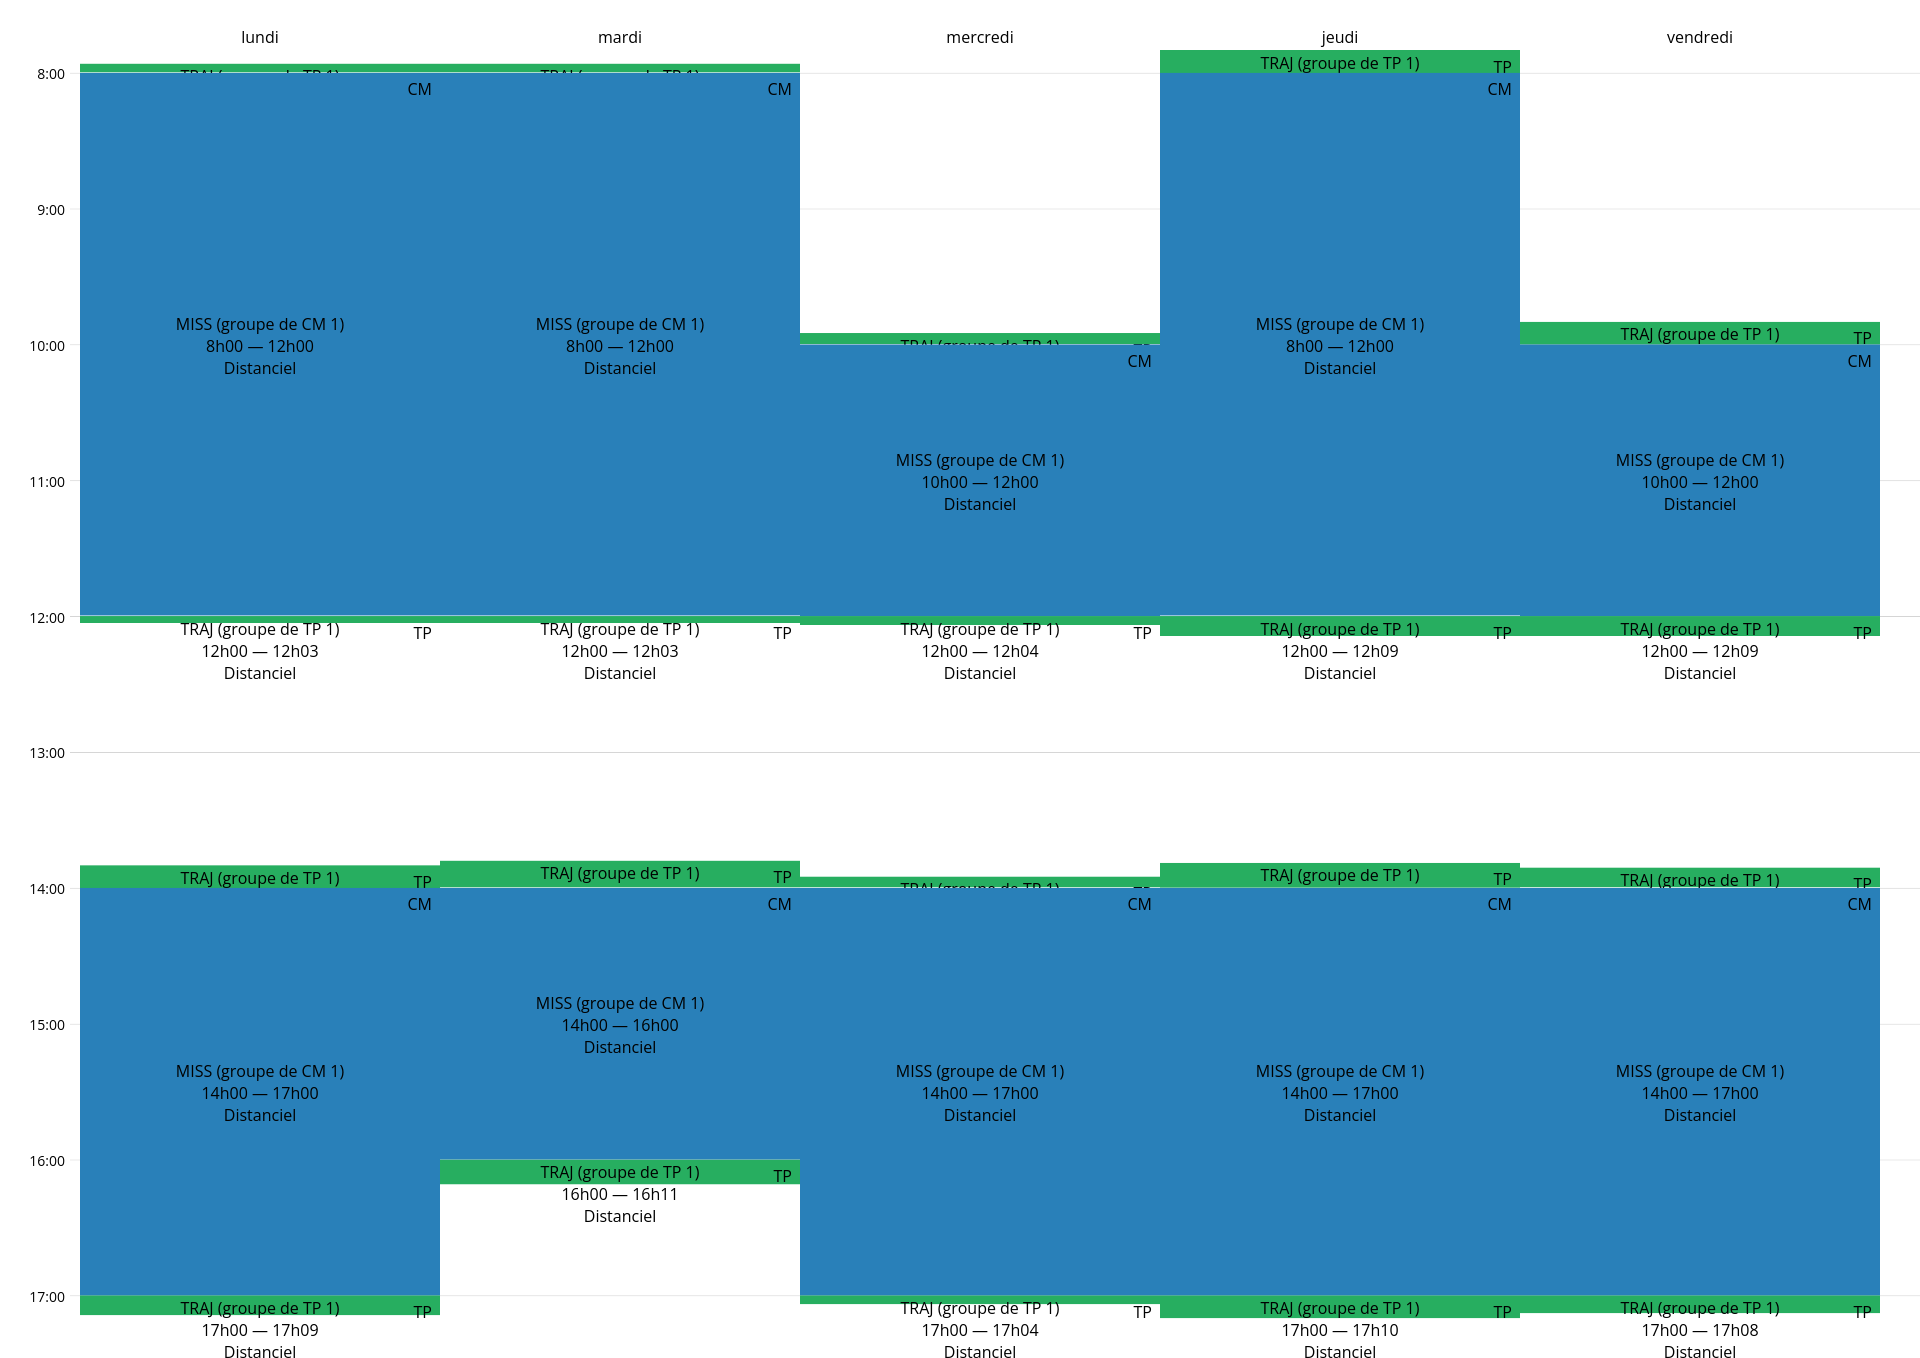
\includegraphics[width=1\textwidth]{Images/edt.png}
    \caption{Image rendue de l'emploi du temps d'un agent}
    \label{fig:edt}
\end{figure}

\newpage
\section{Conclusion}

Nous avons pu mettre en place et implémenter un algorithme cherchant à optimiser les affectations d'agents du SESSAD.
Notre implémentation utilise une heuristique et un algorithme génétique afin d'obtenir une solution initiale, puis utilise l'algorithme de recuit simulé afin de trouver une solution plus optimale.

Nous n'avons pas rencontré de grandes difficulté lors de ces deux étapes, en dehors des problèmes liés à la gestion manuelle du programme, qui a été écrit en C.
La mémoire utilisée par programme a été vérifié avec \texttt{valgrind} et des tests unitaires vérifient le bon fonctionnement des différents composants du programme.

Vous trouverez le code source du projet sur \emph{Github} :\newline \href{https://github.com/kalharko/it45-project}{github.com/kalharko/it45-project}

\subsection{Pistes d'amélioration}
\begin{itemize}
    \item Lorsque le programme est lancé avec plusieurs itérations pour garder la meilleur solution, seul le premier objectif de la cascade est pris en compte pour choisir la meilleur solution.
    \item Génération d'instances du problème complètement intégré au programme à des fins de test.
    \item Plus de tests unitaires.
    \item Comparer différentes manières de calculer les objectifs.
\end{itemize}



\end{document}








